\documentclass[10pt,twocolumn,twoside]{IEEEtran}
\usepackage[T1]{fontenc}
\usepackage{amsmath,amssymb,amsthm}
\usepackage{newtxtext,newtxmath}
\usepackage{graphicx}
\usepackage{booktabs}
\usepackage{array}
\usepackage{multirow}
\usepackage{cite}
\usepackage{xcolor}
\usepackage{url}
\newtheorem{theorem}{Theorem}
\newtheorem{corollary}{Corollary}
\newtheorem{proposition}{Proposition}
\newtheorem{remark}{Remark}
\DeclareMathOperator{\row}{row}
\DeclareMathOperator{\rank}{rank}
\DeclareMathOperator{\col}{col}
\DeclareMathOperator{\nullsp}{null}

\title{When Is Control-Aware Communication Locally Decidable?\\
Information-Structure Limits in Distributed Formation Control}
% HUMAN INPUT REQUIRED BEFORE PORTAL UPLOAD.
% Do not replace these fields with inferred repository metadata.
\author{[VERIFIED AUTHOR LIST REQUIRED]%
\thanks{For every author: [department, institution, complete mailing address,
telephone number, email address, and ORCID required].}%
\thanks{Corresponding author and preferred proof address:
[VERIFIED NAME AND CONTACT REQUIRED].}%
\thanks{Funding and acknowledgments: [VERIFIED STATEMENT OR ``NONE'' REQUIRED].}}


\begin{document}
\maketitle

\begin{abstract}
Control-aware communication assigns resources according to an update's
closed-loop consequence, but a distributed sender may lack the information
needed to determine it.  We study
finite-dimensional sampled linear systems in which a communication action adds
a fixed response to a finite-horizon performance output.  For quadratic cost,
this benefit is an affine functional of an augmented closed-loop state.
Building on functional observability, we characterize exact value
identifiability from current and finite-history agent information by row-space
conditions.  When compatible values straddle zero, we quantify the
irreducible estimation radius and strictly positive local minimax decision
regret for deterministic and randomized sender rules.  For multiple actions,
the minimum instantaneous noiseless linear-statistic dimension is the rank
of the unobservable coefficient projection; algebraic dimension, coalition
ownership, and acquisition cost remain distinct.

We instantiate the framework on sampled formation controllers with delayed and
lossy communication.  A predeclared deterministic registry, frozen before
outcome inspection, spans 72 combinations of 5, 7, and 9 agents, three
connected graphs, two pinning patterns, two horizons, and two delays; its 1320
action functionals are structurally nonidentifiable.  In the frozen five-UAV
instance, for each of ten controller-relevant action types we construct a
nonzero state-generated response admitting an unsaturated, dynamically
reachable history pair with identical allowed sender observations and fixed
responses but opposite exact action-value signs, with independent replay.
Leader action sets share missing-information directions, whereas
tested follower sets do not, and minimum owning coalitions vary with topology.
The results delimit exact local value-based communication without ruling out
prior-specific Bayesian decisions or nonlinear policies.
\end{abstract}

\begin{IEEEkeywords}
Networked control systems, distributed control, information structures,
functional observability, value of information, event-triggered control,
multi-agent formation.
\end{IEEEkeywords}

\section{Introduction}

Communication policies for networked control are increasingly asked to send
the packet that matters most to the control objective, rather than simply the
oldest packet or the packet with the largest state error.  Event-triggered
control formalizes state- or error-dependent transmissions
\cite{tabuada2007event,dimarogonas2012distributed,wang2011eventtriggering};
age of information (AoI) formalizes freshness
\cite{yates2021aoisurvey,rajaraman2021notjustage}; and value-of-information
(VoI) formulations attach a control consequence to an update
\cite{soleymani2023voiglobal}.  These approaches answer different questions.
AoI describes how stale a record is, while a finite-horizon control value asks
how the closed loop will change if that record is refreshed.

The latter question is meaningful only relative to an information structure.
In a distributed formation, the sender knows its own physical and controller
state and its transmission history.  It need not know the packet currently
held by a receiver, the receiver's other stale memories, or remote states that
shape the no-action closed-loop trajectory.  Acknowledgments can reduce one
part of this uncertainty, and ACK-free packet-memory beliefs can be calibrated
under a known channel law.  Neither fact implies that the total control-action
value is locally computable: the cross term between the action response and
the global no-action response may remain hidden.

This paper therefore asks a question prior to scheduler design:

\begin{quote}
Under what information structures is the conditional fixed-response,
finite-horizon benefit of a communication action identifiable, and what
additional information must be acquired when it is not?
\end{quote}

The question connects decentralized information structures
\cite{witsenhausen1971information,ho1972team,nayyar2013common} with functional
observability \cite{fernando2010functional,montanari2022functional}.  We do
not claim the row-space test itself as new.  Rather, we expose the exact
communication-action value as the target functional, show that inability to
observe its magnitude can extend to its sign, separate the dimension of the
missing statistic from the network cost of constructing it, and close these
statements on an implemented formation-control model.

The investigation was driven by falsification.  A deterministic
communication-error bound was analytically valid but produced a Pareto
frontier dominated by periodic communication.  An online centralized
current-state oracle, using the exact action cross term but no future
realizations, exposed substantial scheduling headroom in some nonstationary
regimes and none in a congestion boundary.  Explicit receiver feedback often
consumed that headroom.  Finally, an exact ACK-free receiver-memory belief was
well calibrated but could not identify the baseline component of the action
cross term.  These findings motivated an information-limit result rather than
another trigger.

The contributions are:

\begin{enumerate}
\item We derive the exact finite-horizon marginal communication-action value
as an affine functional of an augmented state for a fixed action response.
\item Using functional-observability geometry, we quantify the irreducible
value-information radius and derive deterministic and randomized local minimax
communication-decision regret when compatible exact values straddle zero.
\item We prove that the minimum dimension of extra instantaneous linear
information for a family of actions is the rank of its hidden projection, and
apply it sender-wise to expose shared versus independent missing directions.
We separately characterize coalition ownership because statistic dimension is
not packet count or distributed acquisition cost.
\item For the sampled formation architecture, a new 72-cell registry across
\(N=5,7,9\), topology, pinning, horizon, and delay yields 1320/1320 structural
nonidentifiability results stable over the declared tolerance grid.  In the
frozen N=5 instance, for each of ten controller-relevant action types we
construct and independently replay an actual state-generated nonzero response
with an opposite-sign witness, quantify heterogeneous practical scale, and
retain the ACK-like break-even diagnostic as acquisition-cost sensitivity only.
\end{enumerate}

The results are scoped to exact affine action-value identifiability in the
stated sampled linear model.  They do not assert that distributed agents can
never make useful stochastic decisions, that feedback is always uneconomic,
or that adaptive communication is universally inferior to periodic service.

\section{Related Work and Positioning}

\subsection{From event conditions to stale receiver memories}

Event-triggered control replaces periodic sampling by state-dependent
conditions while retaining stability or performance guarantees
\cite{tabuada2007event,wang2011eventtriggering,dimarogonas2012distributed,
seyboth2013eventbased,nowzari2019eventtriggered}.  Loss and delay make the
sender and receiver disagree about the control information in use.
Decentralized double-integrator consensus under unreliable links is treated
in \cite{garcia2016unreliable}; ACK and no-ACK event-triggered designs under
packet loss appear in \cite{dolk2017packetlosses}; and model-based triggering
without ACK appears in \cite{garcia2021modelbasedlossy}.  Most closely, Viel
et al. maintain packet-loss hypotheses for neighbor-held states in distributed
formation control \cite{viel2022packetlossformation}.  Thus no-ACK receiver
memory inference is established prior art.  Our issue is what remains hidden
after that receiver-memory uncertainty is represented exactly.

\subsection{Freshness and control value}

AoI measures time since generation of the freshest received update
\cite{yates2021aoisurvey}.  Goal-oriented variants such as age of incorrect
information refine freshness by state relevance
\cite{maatouk2020aoii,rajaraman2021notjustage}; a recent multi-agent overview
organizes goal-oriented communication by the task information being exchanged
\cite{charalambous2026goaloriented}.  These metrics are useful
network summaries but are not generally sufficient statistics for the
finite-horizon marginal value of an action.  VoI-based feedback control makes
that marginal value explicit and can yield optimal threshold structures under
its prescribed information model \cite{soleymani2023voiglobal}.  Recent
finite-horizon scheduling under packet drops likewise uses ACK-derived error
covariance as a fully observed Markov state \cite{yang2026finitehorizon}.
Formation
scheduling has also combined value proxies, graph relevance, and resource
allocation \cite{chiariotti2025voiformation}.  We neither introduce the VoI
concept nor optimize a scheduler.  Bayesian and VoI policies may act optimally
under their stated prior and information model without observing a realized
clairvoyant value.  We instead test the narrower prerequisite for reproducing
the full-information, fixed-response value or its sign at a decision.

\subsection{Information structures and functional observability}

Who knows what and when is central to decentralized control
\cite{witsenhausen1971information,ho1972team}.  Common-information methods can
convert specific partial-history-sharing problems into coordinated stochastic
control problems \cite{nayyar2013common}, but they require a declared
probability model and information sharing architecture.  Multi-agent
return-gap communication clusters local observations using joint action-value
vectors and bounds expected loss relative to full observability
\cite{chen2024rgmcomm}.  That learned stochastic-code problem differs from
exact affine reconstruction, local set-membership regret, and instantaneous
linear-statistic dimension.  Functional
observability asks whether selected linear functionals, rather than the full
state, can be reconstructed \cite{fernando2010functional}.  Its row-space
characterizations and target-estimation questions are established, including
for large networks \cite{montanari2022functional}.  Recent work provides
modal and structural characterizations and optimal sensor-placement results
\cite{zhang2025functionalsensor}, sample-based conditions for intermittent or
irregular measurements \cite{krauss2025samplebased}, and reduced-order
functional-observer existence and pole-placement methods
\cite{darouach2025functional}.  Structural refinements cover generically
diagonalizable systems \cite{zhang2025generic} and fixed-observable-set
characterizations \cite{commault2026note}; target control/observation duality
is developed in \cite{montanari2025duality}.

These results imply three explicit boundaries.  Our current- and
finite-history row-space conditions are applications of functional and
sample-based functional observability, not new generic tests.  Our coalition
search is an instantiated functional sensor-selection problem, not a new
optimization class.  Finally, the instantaneous missing-statistic dimension
derived here is neither minimum sensor count nor functional-observer order.
Our current-state test is specifically an instantaneous functional
reconstructibility application; it is not a functional-observer existence,
detectability, order, or pole-placement result.  Our addition is the
communication-decision consequence: a conditional fixed-response action-value
functional, its local minimax estimation and binary-decision regret, and the
separation between simultaneous-action statistic dimension and network
acquisition cost.

\subsection{Control--communication co-design}

Data-rate theorems and networked-control studies quantify how communication
constrains stability and performance \cite{tatikonda2004control,
nair2007feedback,hespanha2007survey}.  Modern surveys emphasize that
information has several operational meanings in estimation and control
\cite{franceschetti2023manyfacets}.  Feedback itself consumes network
opportunities and can reverse freshness conclusions \cite{munari2025feedback}.
Our break-even analysis is deliberately modest: it asks whether the measured
performance headroom can pay for the messages needed to expose a hidden value
statistic under a frozen packet-frequency accounting model.

\begin{table*}[t]
\caption{Closest research threads and the distinction of this paper.}
\label{tab:prior}
\centering
\scriptsize
\begin{tabular}{p{2.6cm}p{4.1cm}p{4.2cm}p{5.3cm}}
\toprule
Thread & Established capability & Remaining question & Position of this paper \\
\midrule
Event-triggered and lossy formation
& Stability/performance triggers under distributed state error, loss, or delay
& Is exact marginal action value available to the transmitter?
& No new trigger; a valid bound-trigger counterexample motivates the information question. \\
AoI / goal-oriented freshness
& Timeliness and incorrectness metrics
& Does freshness determine the closed-loop action cross term?
& AoI is not treated as a sufficient control-value statistic. \\
VoI scheduling
& Marginal control benefit and threshold scheduling under specified information
& Is the value statistic itself identifiable under a distributed sender map?
& Studies this precondition; makes no optimal-scheduler claim. \\
Decentralized information structures
& Formal dependence of decisions on distributed histories
& Which exact functional is missing for communication decisions?
& Instantiates the information question with finite-horizon communication-action value. \\
Functional and sample-based observability
& Row-space/modal/structural tests, sampling conditions, observer design, and target-sensor selection
& What irreducible value and decision loss follows when a communication-action functional is hidden?
& Uses established tests; adds action-specific minimax regret, simultaneous-action dimension, acquisition separation, and formation closure. \\
\bottomrule
\end{tabular}
\end{table*}

\section{Sampled Distributed Formation and Communication Model}

\subsection{Formation dynamics}

Agent 1 is an analytical leader and
\(\mathcal F=\{2,\ldots,N\}\) are followers.  At sample \(k\), follower i has
position \(p_i\in\mathbb R^3\), velocity \(v_i\in\mathbb R^3\), and input
\(u_i\).  The implemented semi-implicit double-integrator update is
\begin{align}
v_i(k+1)&=v_i(k)+hu_i(k),\\
p_i(k+1)&=p_i(k)+hv_i(k)+h^2u_i(k).
\end{align}
For desired offset \(r_i\), define
\begin{equation}
e_i=p_i-p_1-r_i,\qquad w_i=v_i-v_1.
\end{equation}
The directed convention is \(A_{ij}=1\) when controller i uses a packet sent
by j.  The evaluated graph is fixed and its follower-grounded dynamics are
Schur under the declared gains.  To make the implementation instance explicit,
\begin{equation}
A=\begin{bmatrix}
0&0&0&0&0\\1&0&1&0&0\\0&1&0&1&0\\
0&0&1&0&1\\1&0&0&1&0
\end{bmatrix},\quad
\pi=\begin{bmatrix}0&1&0&1&0\end{bmatrix}^{\!\top},
\label{eq:graph}
\end{equation}
with \(s_i=1\), \(K_p=1.8\), \(K_v=2.2\),
\(K_{pL}=1.5\), and \(K_{vL}=1.8\).

Receiver i stores the newest accepted ordinary neighbor payload
\(\hat x_{ij}=(\hat p_{ij},\hat v_{ij})\).  Pinned followers separately store
\((\hat p^L_{i1},\hat v^L_{i1},\hat a^L_{i1})\).  Newer-generation acceptance
prevents an obsolete reordered packet from replacing newer memory.  DATA may
be lost or delayed; an ACK architecture may separately report acceptance,
but the information-limit theorem only uses the variables actually supplied
to the sender.

Before acceleration saturation, the implemented control law is
\begin{align}
u_i={}&-K_ps_i\sum_jA_{ij}\big[(p_i-\hat p_{ij})-(r_i-r_j)\big]\nonumber\\
&-K_vs_i\sum_jA_{ij}(v_i-\hat v_{ij})
-\pi_iK_{pL}[(p_i-\hat p^L_{i1})-r_i]\nonumber\\
&-\pi_iK_{vL}(v_i-\hat v^L_{i1})+\pi_i\hat a^L_{i1}.
\label{eq:controller}
\end{align}
Its exact-information part is
\(u_F^\star=-H_pe-H_vw+\Pi\mathbf1a_1\); stale memories add a command residual
\(d^c\).  With \(y=\col(e,hw)\), the exact unsaturated sampled update can be
written
\begin{equation}
y_{k+1}=A_hy_k+D_h\col(\chi_k,\upsilon_k),
\label{eq:sampled}
\end{equation}
where \(\chi_k\) is the analytical-leader position-step residual and
\(\upsilon_k=h^2d^c_k+h^2\Pi\mathbf1a_1(k)
-h\mathbf1[v_1(k+1)-v_1(k)]\).  This form follows from the actual
velocity-first integrator; it is not a continuous-time approximation.

\subsection{Information available at a sender}

At a decision by source j, the strongest deterministic local information used
in this paper contains its exact own position and velocity; every ordinary
and pinned receiver memory feeding its own controller; its exact unsaturated
command; graph, gains, offsets, clock, and channel law; and its own sent-DATA
history.  The leader additionally knows its reference position, velocity, and
acceleration.  It does not include state stored at another receiver or remote
physical state that has not been communicated.  We express the state-dependent
part as
\begin{equation}
o_j=C_j\xi+d_j.
\label{eq:sender-map}
\end{equation}
Known packet histories or action labels change affine constants but do not add
hidden-state rows.  Figure~\ref{fig:architecture} illustrates the distinction.

\begin{figure}[t]
\centering
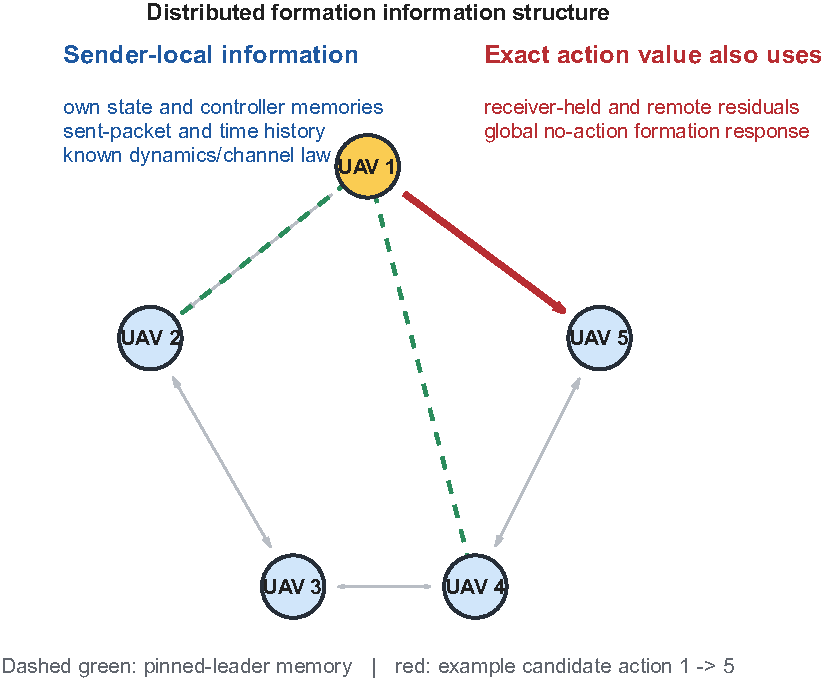
\includegraphics[width=\columnwidth]{figures/fig1_information_architecture.pdf}
\caption{Evaluated distributed information architecture.  The exact value of
the highlighted candidate depends on the global no-action response, not only
on the sender's own state and estimate of receiver memory.}
\label{fig:architecture}
\end{figure}

\section{Finite-Horizon Value of a Communication Action}

\subsection{Generic linear/affine closed loop}

Consider a finite-dimensional affine closed loop
\begin{equation}
x_{k+1}=Ax_k+Bu_k+d.
\end{equation}
For a fixed decision point, collect the no-action performance output over a
finite horizon as
\begin{equation}
z=Fx+r.
\label{eq:baseline}
\end{equation}
A candidate communication action a induces a fixed response \(g_a\) in the
same stacked output.  With symmetric \(Q\succeq0\), define benefit as
no-action cost minus action cost:
\begin{align}
q_a(x)&=\|Fx+r\|_Q^2-\|Fx+r+g_a\|_Q^2\nonumber\\
&=\ell_a^\top x+c_a,
\label{eq:affine-value}
\end{align}
where
\begin{equation}
\ell_a=-2F^\top Qg_a,\qquad
c_a=-2r^\top Qg_a-g_a^\top Qg_a.
\label{eq:value-coeff}
\end{equation}
Positive normalizations, including a delivery probability, do not change
identifiability or sign.  If the response depends on an unknown state, that
state must be augmented or the response must be conditioned on a hypothesis;
otherwise \eqref{eq:affine-value} does not apply.
This quantity is a conditional, fixed-response, finite-horizon marginal
output-cost benefit.  It freezes the decision point, no-action baseline,
controller, horizon, and candidate response; it is not a Bellman value,
state-action \(Q\)-function, or general stochastic VoI that reoptimizes future
controls, schedules, or channel outcomes.

\subsection{Formation action response}

For the formation case, the augmented state contains exactly the variables
needed to construct the frozen no-action response: follower formation error
and scaled relative velocity, analytical-leader state, eight ordinary
receiver memories, and two pinned-leader memories.  For one Cartesian axis,
\begin{equation}
\begin{aligned}
\xi^a=\col\!\big(&e^a,hw^a,p_L^a,hv_L^a,h^2a_L^a,\\
&\{\hat p_{ij}^a,h\hat v_{ij}^a\},\\
&\{\hat p_{iL}^a,h\hat v_{iL}^a,h^2\hat a_{iL}^a\}\big).
\end{aligned}
\label{eq:aug-state}
\end{equation}
The one-axis dimension is 33 and
\(\xi=\col(\xi^x,\xi^y,\xi^z)\in\mathbb R^{99}\).

Recursion of \eqref{eq:sampled} over H samples yields implementation-derived
matrices, not fitted matrices,
\begin{equation}
\operatorname{vec}(Z_k)=F_H\xi_k+r_H.
\label{eq:FH}
\end{equation}
For link \(j\to i\), receiver-memory hypothesis s, successful-delivery
probability \(p_s\), \(m=N-1\), and fixed output response \(g_{ij,s}\),
\begin{equation}
q_{ij,s}=-\frac{2p_s}{m}g_{ij,s}^\top(F_H\xi_k+r_H)
-\frac{p_s}{m}\|g_{ij,s}\|_2^2.
\label{eq:formation-value}
\end{equation}
Here \(Z_k\) stacks H sampled follower-position errors.  Consequently
\(q_{ij,s}\) is a per-follower sum of squared sampled position-error
differences, measured in \(\mathrm{m}^2\); it is not an RMSE or
time-integrated mission cost.
For a receiver-memory belief \(b(s)\), the exact conditional expression is
\(\bar q_{ij}=\sum_s b(s)q_{ij,s}\).  The coefficient and constant are
averaged across hypotheses.  We do not evaluate the nonlinear quadratic at
an expected receiver state.  When \(\xi_k\) contains components hidden from
the sender, this receiver-memory marginalization is not
\(\mathbb E[q\mid\mathcal I_j]\) unless an additional joint state prior is
specified.

\section{Information-Structure Identifiability}

\subsection{Static current-value reconstructibility}

The following classical row-space fact is specialized to the conditional
fixed-response communication benefit.  It is used as a prerequisite, not
claimed as a new functional-observability theorem.

\begin{theorem}[Static fixed-response action-value identifiability]
\label{thm:exact}
Let \(q_a(x)=\ell_a^\top x+c_a\) and \(o=Cx+d_o\).  On
\(\mathbb R^n\), or locally on a feasible set containing an open relative
neighborhood along \(\ker C\), the exact action value is a function of o if
and only if
\begin{equation}
\ell_a\in\row(C).
\label{eq:row-test}
\end{equation}
\end{theorem}

\begin{proof}
If \(\ell_a=C^\top\alpha\), then
\(q_a=\alpha^\top(o-d_o)+c_a\).  Conversely, any \(v\in\ker C\) leaves o
unchanged.  Identifiability requires
\(q_a(x+v)-q_a(x)=\ell_a^\top v=0\) for every such v.  Hence
\(\ell_a\in(\ker C)^\perp=\row(C)\).
\end{proof}

The normalized diagnostic used later is
\begin{equation}
\delta_C(\ell)=
\frac{\|(I-C^\dagger C)\ell\|_2}{\max(\|\ell\|_2,\epsilon)}.
\label{eq:residual}
\end{equation}
A positive numerical residual applies the theorem to a given matrix; it is
not itself the theorem.

\subsection{Finite local history}

Suppose that during a declared interval the augmented dynamics and
measurements are
\begin{equation}
x_{t+1}=A_0x_t+a_0,\qquad o_t=Cx_t+d.
\end{equation}
Define
\begin{equation}
\mathcal O_L=\col(C,CA_0,\ldots,CA_0^L).
\end{equation}

\begin{theorem}[Finite-history action-value identifiability]
\label{thm:history}
At time L, an action value with coefficient \(\ell_a\) is identifiable from
\(o_0,\ldots,o_L\) if and only if
\begin{equation}
(A_0^L)^\top\ell_a\in\row(\mathcal O_L).
\label{eq:history-test}
\end{equation}
After the observability row space has stabilized, later samples add no
observation direction.  They cannot recover a decision-time value whenever
its propagated coefficient remains outside that stabilized row space.
\end{theorem}

\begin{proof}
The affine solution gives
\(x_L=A_0^Lx_0+\sum_{t=0}^{L-1}A_0^{L-1-t}a_0\).  Thus the coefficient of
the time-\(L\) value in \(x_0\) is \((A_0^L)^\top\ell_a\), while the stacked history's
state-dependent part is \(\mathcal O_Lx_0\).  Theorem~\ref{thm:exact} gives
\eqref{eq:history-test}.  Cayley--Hamilton implies that the row span generated
by \(C,CA_0,\ldots\) stabilizes in finite dimension.
\end{proof}

This is the corresponding sampled functional-observability specialization,
not a new result based merely on sampling.  The last sentence is conditional
on unchanged maps and a coefficient that
retains its hidden component.  A hidden mode annihilated by the dynamics can
cease to affect a later value; that is loss of dependence, not recovery of
information.  A delivered packet, new sensor, or shared statistic changes the
information structure.

\subsection{Irreducible value and decision uncertainty}

Exact magnitude is stronger than the sign needed by a transmit-if-beneficial
rule.  Let \(\mathcal X\) be the declared operating set,
\begin{equation}
\mathcal X(o)=\{x\in\mathcal X:Cx+d_o=o\},
\end{equation}
and assume its image under \(q\) is a nonempty closed finite interval
\begin{equation}
\mathcal Q(o)=[q_-(o),q_+(o)].
\end{equation}
Define the midpoint and value-information radius
\begin{equation}
q_c(o)=\frac{q_+(o)+q_-(o)}2,\qquad
\Delta_q(o)=\frac{q_+(o)-q_-(o)}2.
\label{eq:value-radius}
\end{equation}

\begin{theorem}[Irreducible value and communication-decision uncertainty]
\label{thm:sign}
At a fixed information state \(o\):
\begin{enumerate}
\item the minimax error of any sender-local point estimate is
\begin{equation}
\inf_{\widehat q(o)}\sup_{x\in\mathcal X(o)}
|\widehat q(o)-q(x)|=\Delta_q(o),
\label{eq:minimax-value}
\end{equation}
and the midpoint \(\widehat q=q_c\) is optimal;
\item if \(q_-<0<q_+\), no deterministic map of \(o\) recovers the exact value
sign for every compatible state;
\item for a binary decision whose exact-information rule transmits iff
\(q>0\), a sender-local randomized rule transmitting with probability \(p\) has
local endpoint regrets
\begin{equation}
R_+(p)=(1-p)q_+,\qquad R_-(p)=p(-q_-).
\end{equation}
Its minimax probability and unavoidable regret are
\begin{equation}
p^*=\frac{q_+}{q_++(-q_-)},\qquad
R_{\rm rand}^*=\frac{q_+(-q_-)}{q_++(-q_-)}>0.
\label{eq:random-regret}
\end{equation}
Restricting to deterministic rules gives
\begin{equation}
R_{\rm det}^*=\min\{q_+,-q_-\}>0.
\label{eq:det-regret}
\end{equation}
\end{enumerate}
\end{theorem}

\begin{proof}
For any scalar estimate \(y\),
\(q_+-q_-\le |q_+-y|+|y-q_-|\), so its worst endpoint error is at least
\((q_+-q_-)/2\); the midpoint attains that bound throughout the interval.
If the interval straddles zero, the same observation is compatible with
opposite exact signs, proving the deterministic statement.  For the randomized
action, regret over positive values is maximized at \(q_+\) and decreases with \(p\);
regret over negative values is maximized at \(q_-\) and increases with \(p\).  Equating
\((1-p)q_+=p(-q_-)\) yields \eqref{eq:random-regret}.  The deterministic
choices \(p=0\) and \(p=1\) incur worst regrets \(q_+\) and \(-q_-\), respectively, proving
\eqref{eq:det-regret}.
\end{proof}

The strict-straddling formulas above have transparent boundary cases.  If
\(q_-=0<q_+\), choosing \(p=1\) gives zero minimax regret; if
\(q_-<0=q_+\), choosing \(p=0\) does so; and if both endpoints are zero every
choice has zero regret.  A non-straddling interval admits a deterministic
common-sign decision with zero regret.  For the symmetric interval
\([-a,a]\), \(p^*=1/2\), \(R_{\rm rand}^*=a/2\), and
\(R_{\rm det}^*=a\).  If transmission instead requires a net benefit above
threshold \(\tau\), apply the same theorem to
\(v=q-\tau\) and the shifted interval
\([q_--\tau,q_+-\tau]\).  The formation witnesses below use \(\tau=0\).

For \(q(x)=a^\top x+b\), let
\(P_C=C^\dagger C\), \(a_\perp=(I-P_C)a\), and consider the Euclidean local
fiber \(x=x_0+v\), \(v\in\ker C\), \(\|v\|_2\le\rho\).  Its exact interval is
\begin{equation}
\begin{aligned}
\mathcal Q(o)&=[q(x_0)-\rho\|a_\perp\|_2,\\
&\quad q(x_0)+\rho\|a_\perp\|_2],\\
\Delta_q(o)&=\rho\|a_\perp\|_2.
\end{aligned}
\label{eq:sign-interval}
\end{equation}
The endpoints follow by choosing \(v\) parallel or antiparallel to
\(a_\perp\).  Figure~\ref{fig:geometry} shows the geometry.

Theorem~\ref{thm:sign} is a local minimax statement over \(\mathcal X(o)\),
not a universal stochastic-control lower bound.  It does not rule out a
Bayesian conditional expectation under a specified prior, nor does it say
that every information fiber crosses zero.

\section{Minimum Supplementary Information and Coalition Structure}

\subsection{One or multiple candidate actions}

Stack \(p\) action-value coefficients as rows of
\(L\in\mathbb R^{p\times n}\) and define
\begin{equation}
L_\perp=L(I-C^\dagger C).
\label{eq:Lperp}
\end{equation}

\begin{theorem}[Minimum instantaneous linear-statistic dimension]
\label{thm:min-stat}
Under an instantaneous, noiseless, arbitrary-precision real-valued linear
supplementary map \(Hx\), the minimum number of scalar rows required to
identify all \(p\) exact action values is
\begin{equation}
r_\star=\rank(L_\perp).
\label{eq:rstar}
\end{equation}
\end{theorem}

\begin{proof}
If all values are identifiable from \(\col(C,H)x\), the projections of the
rows of \(H\) onto \(\ker C\) must span every row of \(L_\perp\).  Therefore \(H\)
has at least \(\rank(L_\perp)\) independent scalar rows.  Conversely, choose
the rows of \(H\) as any row basis of \(L_\perp\).  Each row of \(L\) is then the sum
of a component in \(\row(C)\) and one in \(\row(H)\), satisfying
Theorem~\ref{thm:exact} for all \(p\) values.
\end{proof}

For a single nonidentifiable value, one additional scalar
\(\theta=\ell_\perp^\top x\) is sufficient.  This is statistic dimension,
not packet count.  The coordinates of \(\ell_\perp\) may be distributed
across many agents.

\begin{corollary}[Instantaneous linear supplementary statistics]
\label{cor:message-dimension}
Under the same noiseless arbitrary-precision linear model, if the decision
maker can receive \(r\) independent real-valued scalar statistics before
deciding, exact identification of all \(p\) values requires
\(r\ge r_\star\).  Equality is algebraically achievable if those statistics
span \(\row(L_\perp)\).
\end{corollary}

This is a linear-statistic-dimension statement, not a data-rate theorem.  Scalar
dimension, packet count, bits, latency, functional-observer order, and the
distributed cost of synthesizing each scalar are distinct quantities.

\subsection{Information ownership}

Let agent \(i\)'s strongest map be \(C_i\).  For coalition \(\mathcal S\), define
\(C_{\mathcal S}=\col_{i\in\mathcal S}C_i\).

\begin{corollary}[Coalition identifiability]
\label{cor:coalition}
Coalition \(\mathcal S\) identifies a fixed action value if and only if
\begin{equation}
\ell\in\row(C_{\mathcal S}).
\end{equation}
A minimum owning coalition solves
\begin{equation}
\min_{\mathcal S}|\mathcal S|
\quad\text{subject to}\quad
\ell\in\row(C_{\mathcal S}).
\label{eq:coalition}
\end{equation}
\end{corollary}

Corollary~\ref{cor:coalition} is closely related to functional sensor
selection.  We exhaustively enumerate only the finite evaluated registry
through N=9 and claim no new generic combinatorial algorithm.
Even when a coalition owns the required rows, a causal aggregation protocol
must still communicate them at a nonzero frequency, delay, and reliability
cost.

\section{Communication Cost of Acquiring Value Information}

Let \(C_P(E)\) be the cost of the frozen periodic Pareto frontier interpolated
at formation error \(E\).  Suppose a policy informed by supplementary statistics
uses DATA cost \(D\) and information streams \(t\) with rate \(R_t\) and normalized
price \(\eta_t\).  A necessary accounting condition for performance-matched
Pareto benefit is
\begin{equation}
D+\sum_t\eta_tR_t<C_P(E).
\label{eq:econ-general}
\end{equation}
For a single feedback stream with rate \(A\),
\begin{equation}
\eta^\star=\frac{C_P(E)-D}{A}
\label{eq:eta-star}
\end{equation}
is its break-even price.  Negative \(\eta^\star\) means DATA alone is already
more costly than periodic at matched error.  At feedback price \(\eta_f\), the
affordable feedback fraction is \(f^\star=\eta^\star/\eta_f\), clipped to
\([0,1]\) for operational interpretation.

Equation~\eqref{eq:econ-general} is not an optimality theorem.  It prevents a
common category error: a one-dimensional sufficient statistic is not free.
Under a packet-frequency metric, piggybacking adds no packet only if an
existing packet is sent anyway; bytes, airtime, collision risk, and joules
remain outside that metric.

\section{Formation-Control Case Study}

% Declare the six main evidence figures in their preregistered order.  Their
% interpretation follows in the case-study subsections below.
\begin{figure}[t]
\centering
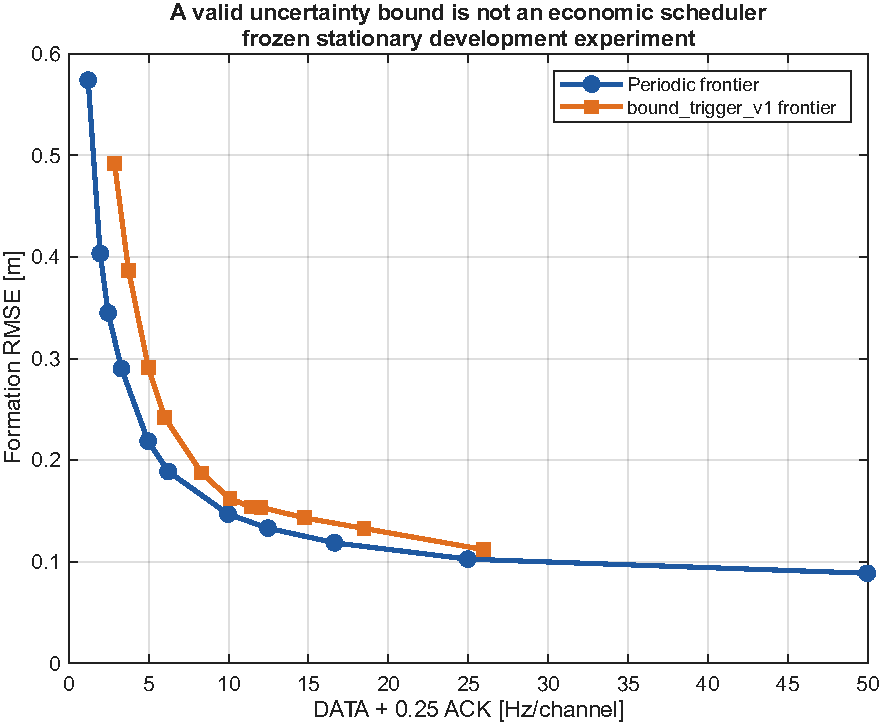
\includegraphics[width=\columnwidth]{figures/fig2_bound_trigger_falsification.pdf}
\caption{Frozen stationary frontiers from five paired development seeds.
The analytically valid bound-based mechanism is dominated by the periodic
frontier over their shared domain.  The comparison is descriptive, not a
population claim.}
\label{fig:bound}
\end{figure}

\begin{figure*}[t]
\centering
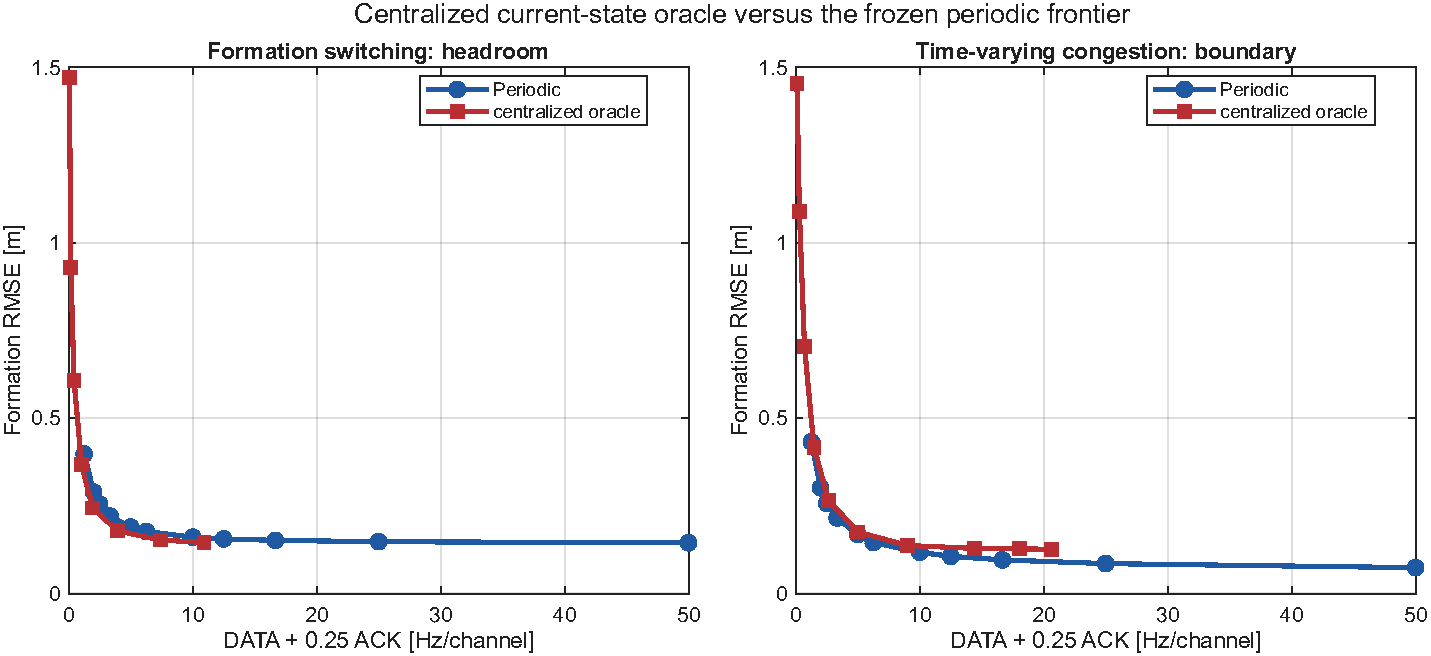
\includegraphics[width=0.96\textwidth]{figures/fig3_oracle_headroom_boundary.pdf}
\caption{Frozen five-seed development diagnostic with centralized current
plant and receiver information.  The conditional fixed-response value creates
Pareto headroom in S2 but not in the S4 congestion boundary.  The oracle is
privileged and nondeployable, and the comparison is non-inferential.}
\label{fig:oracle}
\end{figure*}

\begin{figure}[t]
\centering
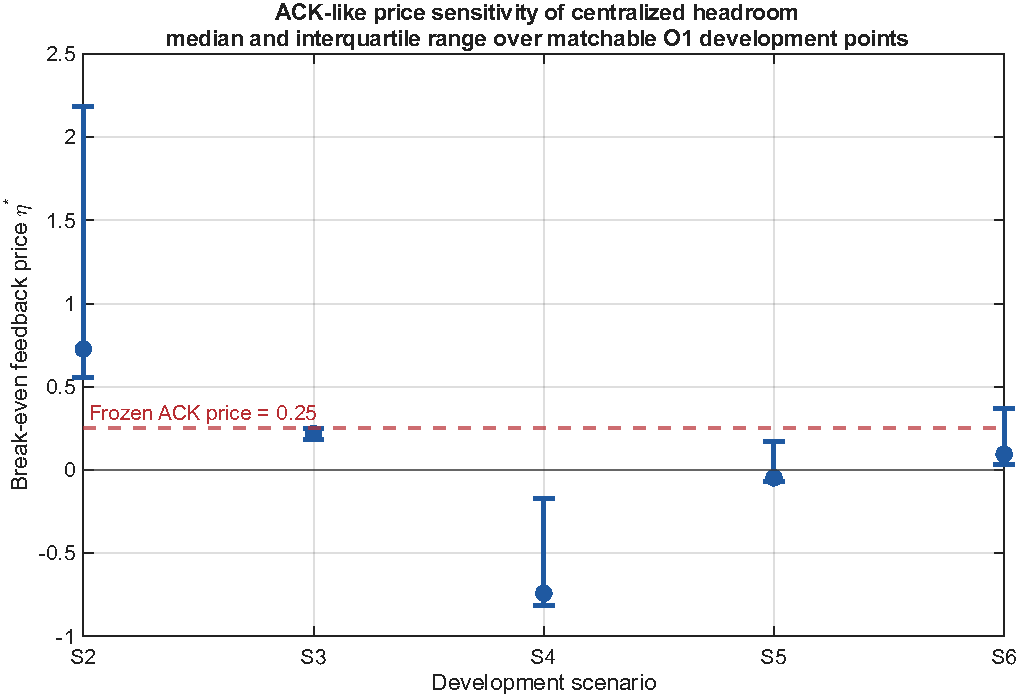
\includegraphics[width=\columnwidth]{figures/fig4_feedback_economics.pdf}
\caption{ACK-like packet-frequency cost sensitivity over frozen,
performance-matchable centralized-oracle development points (median and IQR).  The dashed
line is the preregistered price 0.25.  This does not measure the cost of
acquiring the all-agent missing statistic.}
\label{fig:economics}
\end{figure}

\begin{figure}[t]
\centering
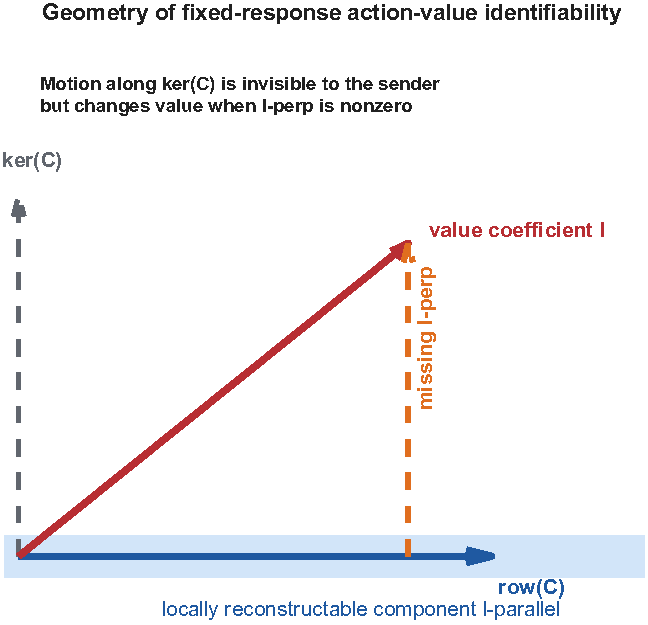
\includegraphics[width=\columnwidth]{figures/fig5_information_geometry.pdf}
\caption{The available row space determines the reconstructable component of
the value coefficient.  Motion along the information null space is invisible
to the sender but changes value when the missing projection is nonzero.}
\label{fig:geometry}
\end{figure}

\subsection{Implementation-derived matrices and cross-instance validation}

The frozen case uses N=5, \(h=0.02\) s, four followers, eight ordinary
controller links, two pinned-leader streams, H=25, and D=4 samples.  Its
augmented state has 33 entries per axis and 99 in 3-D.  The matrices \(F_H\),
action responses, sender maps, and held-memory dynamics are assembled directly
from the implemented graph, gains, controller, and integrator.  For each
controller-relevant payload, a structural command correction
\([1,0,0]^\top\) and fixed receiver-memory hypothesis define \(g\).  The
maximum discrepancy between the affine representation and the centralized
calculation is \(4.34\times10^{-16}\).

To test whether the information-structure observation is peculiar to that
instance, we froze a new Cartesian registry before viewing its results:
\(N\in\{5,7,9\}\), three deterministic connected graphs, even/odd follower
pinning, \(H\in\{15,25\}\), and \(D\in\{2,4\}\).  All 72 configurations
satisfy the same symmetric grounded Schur scope.  Fixed-payload histories use
the complete finite-dimensional horizon \(n_{\rm free}-1\).  Before grounding,
ring2 is a cycle, sparse4 adds cyclic distance-two edges, and geometric is the
first connected radius graph on the deterministic lattice in the sequence
0.60, 0.75, \(\ldots\) m.
Table~\ref{tab:links} summarizes all 1320 action rows.

\begin{table*}[t]
\caption{Cross-instance structural audit. ``Rows'' aggregates two pinning
patterns, two H values, and two D values; every row is nonidentifiable, stable
in membership over relative tolerances \(10^{-6}\)--\(10^{-14}\).  After the
retained row space is orthonormalized and the value row is normalized, every
value row adds one dimension. ``Raw stable'' counts rows whose unnormalized
information-map rank itself does not change over that grid.}
\label{tab:links}
\centering
\scriptsize
\begin{tabular}{llrrrrl}
\toprule
Graph & N & Rows/non-ID & Raw stable & Leader $(p_1,r_1^*)$ & $r_1^*/p_1$ & Minimum coalition pattern \\
\midrule
geometric & 5 & 48/48 & 48 & (6,4) & 0.667 & leader: 5 \\
ring2 & 5 & 80/80 & 56 & (4,3) & 0.750 & every sender: 5 \\
sparse4 & 5 & 144/144 & 96 & (6,4) & 0.667 & every sender: 5 \\
geometric & 7 & 104/104 & 80 & (7,5) & 0.714 & leader: 7; followers: 5 \\
ring2 & 7 & 120/120 & 80 & (5,4) & 0.800 & every sender: 7 \\
sparse4 & 7 & 216/216 & 56 & (7,5) & 0.714 & every sender: 7 \\
geometric & 9 & 160/160 & 80 & (8,6) & 0.750 & leader: 9; followers: 8 \\
ring2 & 9 & 160/160 & 48 & (6,5) & 0.833 & every sender: 9 \\
sparse4 & 9 & 288/288 & 64 & (8,6) & 0.750 & every sender: 9 \\
\bottomrule
\end{tabular}
\end{table*}

At \(10^{-10}\), compressed-null and independent direct-row-space calculations
agree for 1320/1320 rows; the normalized hidden residual spans
\(3.03\times10^{-6}\)--0.99999.  Across the tolerance grid, raw rank is stable
for only 608/1320 rows and raw \(\rank([C;\ell^\top])\) adds one in 1222 rows at
\(10^{-6}\) and 614 at \(10^{-14}\).  An independent reconstruction matches all
6600 stored decisions, while normalized-basis augmentation gives 1320/1320 at
every cutoff.  Selected 80-digit checks, including each cell's minimum,
remain positive.  The claim is therefore scale-controlled functional
membership in a finite registry, not invariant raw-rank bookkeeping or an
arbitrary-graph/gain theorem.

The structural correction fixes \(g\) and must not be confused with a
trajectory-realized scheduling action.  Zero response has zero value, and
special nonzero responses can cancel a hidden projection.  The next subsection
therefore audits actual state-generated corrections separately.

\subsection{Reachable value-sign witnesses}

Affine nonidentifiability alone could be dismissed as an inadmissible state
perturbation.  We therefore audit each of the ten controller-relevant action
types in the frozen N=5 catalog.  Receiver memories are initialized
consistently and held without a DATA update until the decision.  A deterministic source excitation
creates an actual 0.01 m/s$^2$ x-axis controller correction.  For follower
senders, the larger of the source's position and scaled-velocity transfers is
used; leader actions use constant velocity.  We then project the exact
fixed-response value gradient into the consistent-initialization subspace that
simultaneously preserves the complete sender history, target receiver memory,
and actual action response.  Symmetric perturbations about the exact affine
zero crossing are replayed through the implemented controller and integrator.

For each of the ten catalog action types, an actual state-generated nonzero
response yields an admissible opposite-sign pair; six have follower senders
not covered by the earlier representative construction.
Independent replay from persisted coordinates recomputes the physical
controller and centralized trajectories rather than reusing the affine sign
expression.  Correction, payload, branch, and response match within every
pair.  Maximum history, dynamic, and affine-versus-oracle residuals are
\(7.98\times10^{-20}\), \(4.17\times10^{-16}\), and
\(4.07\times10^{-20}\); response mismatch is zero.  The \(10^{-4}\)
coordinate half-separation yields a smallest endpoint \(8.52\times10^{-8}\),
over \(8.5\times10^4\) sign tolerances, and minimum saturation margin 0.952
m/s$^2$.  Values in
Table~\ref{tab:regret} are in \(\mathrm{m}^2\) under the sampled per-follower
normalization following \eqref{eq:formation-value}.

\begin{table*}[t]
\caption{N=5 actual-action reachable value-sign witnesses.  The normalized
radius divides \(\Delta_q\) by the median absolute exact value on a deterministic
32-state local grid. ``Cross'' is the fraction of those states whose radius-
\(10^{-4}\) compatible interval crosses zero; it is descriptive, not a
population probability.}
\label{tab:regret}
\centering
\scriptsize
\begin{tabular}{lrrrrr}
\toprule
Action & $q_-$ & $q_+$ & $\Delta_q$ & Normalized radius & Cross \\
\midrule
ordinary $1\to2$ & $-3.475\times10^{-6}$ & $3.475\times10^{-6}$ & $3.475\times10^{-6}$ & 0.1590 & 0.1875 \\
ordinary $1\to5$ & $-5.344\times10^{-6}$ & $5.344\times10^{-6}$ & $5.344\times10^{-6}$ & 0.1953 & 0.0625 \\
ordinary $2\to3$ & $-5.392\times10^{-6}$ & $5.392\times10^{-6}$ & $5.392\times10^{-6}$ & 0.01010 & 0.09375 \\
ordinary $3\to2$ & $-8.519\times10^{-8}$ & $8.519\times10^{-8}$ & $8.519\times10^{-8}$ & 0.0002666 & 0 \\
ordinary $3\to4$ & $-3.198\times10^{-6}$ & $3.198\times10^{-6}$ & $3.198\times10^{-6}$ & 0.009173 & 0.0625 \\
ordinary $4\to3$ & $-5.223\times10^{-6}$ & $5.223\times10^{-6}$ & $5.223\times10^{-6}$ & 0.01080 & 0 \\
ordinary $4\to5$ & $-1.333\times10^{-7}$ & $1.333\times10^{-7}$ & $1.333\times10^{-7}$ & 0.0003459 & 0 \\
ordinary $5\to4$ & $-3.396\times10^{-6}$ & $3.396\times10^{-6}$ & $3.396\times10^{-6}$ & 0.01099 & 0.0625 \\
pin $1\to2$ & $-3.449\times10^{-6}$ & $3.449\times10^{-6}$ & $3.449\times10^{-6}$ & 0.2315 & 0.2500 \\
pin $1\to4$ & $-5.002\times10^{-6}$ & $5.002\times10^{-6}$ & $5.002\times10^{-6}$ & 0.2106 & 0.03125 \\
\bottomrule
\end{tabular}
\end{table*}

Because the endpoints are centered symmetrically, Theorem~\ref{thm:sign} gives
\(p^*=1/2\), randomized minimax regret \(\Delta_q/2\), and deterministic
minimax regret \(\Delta_q\) for every row.  These are local one-decision losses,
not expected mission-level bounds.  Practical scale is heterogeneous: the
normalized radius exceeds 0.15 for both pin and both leader ordinary actions,
but is below \(3.5\times10^{-4}\) for two follower actions.  Seven of ten
actions cross zero somewhere on the selected 32-state grid; a constructed
reachable witness exists for each catalog type.  The maximum is 0.232, or
0.145 and 0.175 under RMS and IQR/1.349 scaling; the two smallest remain
order \(10^{-4}\).  Figure~\ref{fig:witness} shows this heterogeneity.

\begin{figure*}[t]
\centering
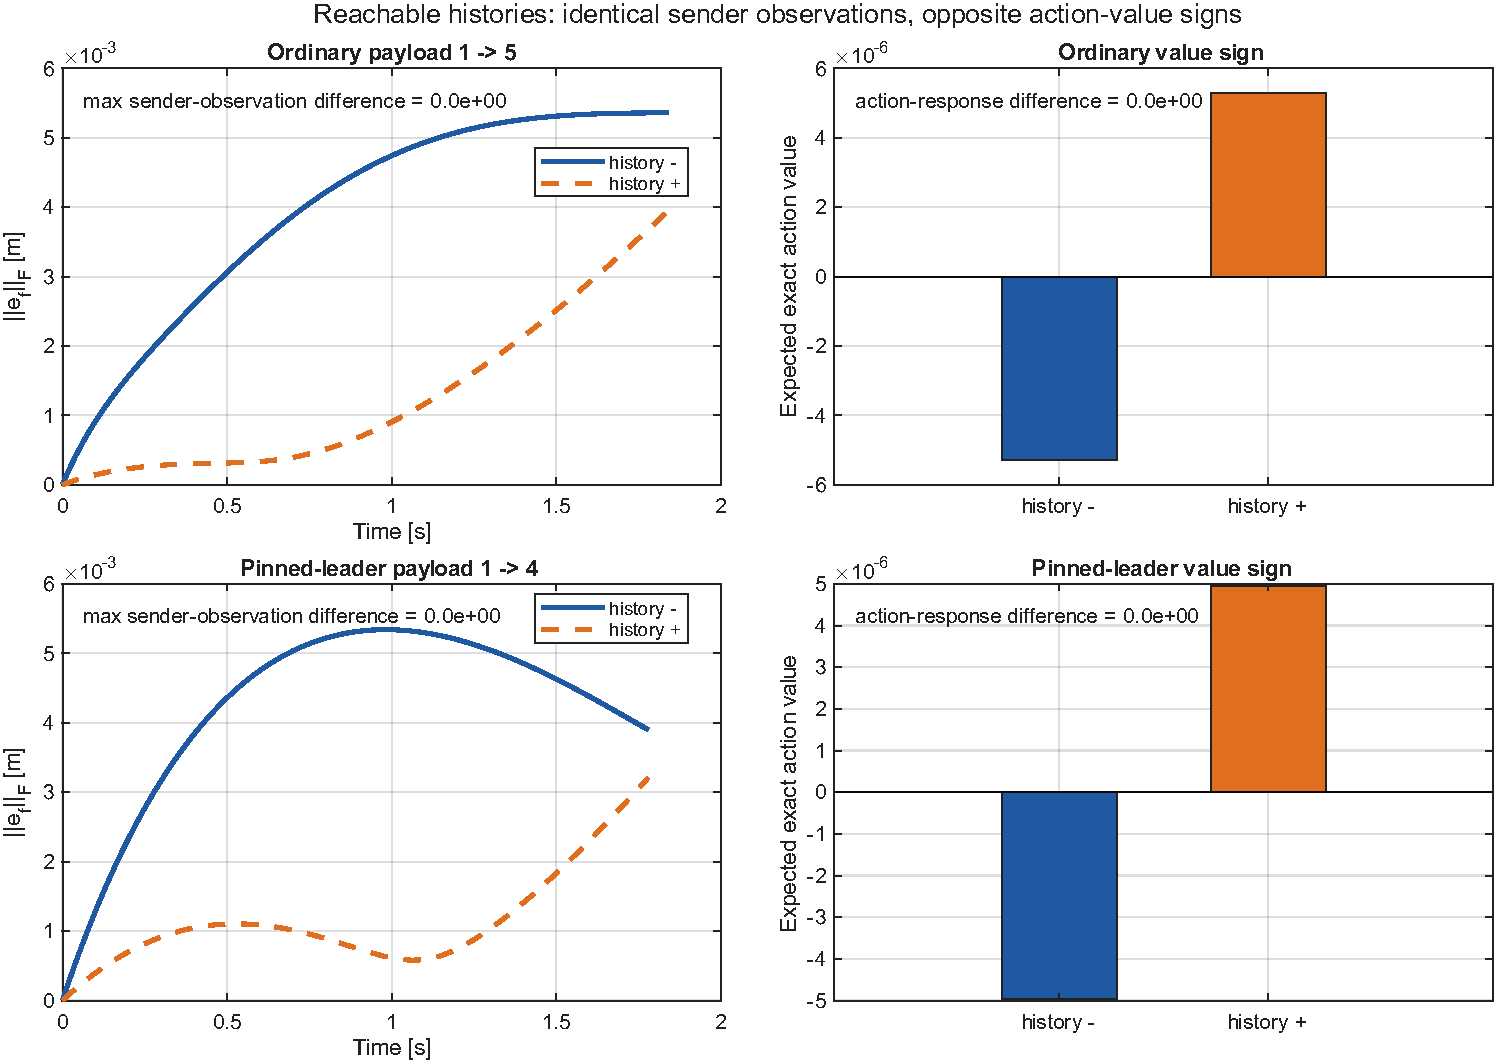
\includegraphics[width=0.84\textwidth]{figures/fig6_reachable_sign_witnesses.pdf}
\caption{Implementation-replayed N=5 actual-action witnesses.  Left: one
constructed actual-response pair for each of ten catalog action types.  Right:
local information radius normalized by typical exact action-value scale; labels
give the deterministic-grid zero-crossing fraction.  Small normalized radius
for some actions is retained rather than interpreted as uniform practical impact.}
\label{fig:witness}
\end{figure*}

\subsection{Statistic dimension versus coalition size}

For every fixed payload, \(\rank(L_\perp)=1\): one linear scalar closes its
individual algebraic deficit.  However, no receiver alone and no
sender--receiver pair identifies that scalar.  Exhaustive enumeration of all
subsets of the five implemented agent maps finds that every sender needs four
additional agents; the only minimum coalition contains all five UAVs.  This
is conditioned on the evaluated graph, H=25, the selected global stacked
formation-error output with identity weighting, and the declared current
information maps.  A localized or decomposable objective can yield a smaller
coalition.  It is not a claim that all formations require global information.

The fixed-action statement underuses Theorem~\ref{thm:min-stat}.  We therefore
stack every controller-relevant current action of each actual sender in
\(L_j\), using a common full 99-dimensional state and the structural unit
command response.  Table~\ref{tab:multi-action} reports the simultaneous
missing rank.  Sender 1 has four payloads but \(r_1^*=3\): its ordinary and
pinned-leader unit actions into follower 2 induce the same output-response
direction, so one hidden direction is shared.  Senders 3 and 4 each require
two independent directions for two actions; the single-action senders require
one.  Thus compression exists for the leader but is not universal.  The
nonzero singular values shown in the table are those of
\(L_j(I-C_j^\dagger C_j)\).

\begin{table*}[t]
\caption{Sender-wise simultaneous-action missing dimension and ownership.}
\label{tab:multi-action}
\centering
\scriptsize
\begin{tabular}{rrrrp{6.5cm}ll}
\toprule
Sender j & $p_j$ & $r_j^*$ & $r_j^*/p_j$ & Retained singular values of $L_j^\perp$ & Minimum coalition & Interpretation \\
\midrule
1 & 4 & 3 & 0.75 & 26.9758; 20.5237; 1.83164 & $\{1,2,3,4,5\}$ & one shared direction \\
2 & 1 & 1 & 1.00 & 49.7427 & $\{1,2,3,4,5\}$ & single action \\
3 & 2 & 2 & 1.00 & 55.0690; 16.5170 & $\{1,2,3,4,5\}$ & independent directions \\
4 & 2 & 2 & 1.00 & 61.7396; 5.34031 & $\{1,2,3,4,5\}$ & independent directions \\
5 & 1 & 1 & 1.00 & 45.7777 & $\{1,2,3,4,5\}$ & single action \\
\bottomrule
\end{tabular}
\end{table*}

Although \(r_1^*=3<4\), the minimum coalition for its entire missing subspace
still contains all five agents.  The same coalition size holds for every
other sender's full action set.  Compression of value directions therefore
does not imply local ownership or three packets: Corollary~\ref{cor:message-dimension}
counts independent real-valued statistics only if their operands can be
assembled before the decision.

The cross-instance audit qualifies the ownership result.  Leader compression
recurs in every registry cell: \(r_1^*/p_1\) ranges from 2/3 to 5/6, while every
tested follower has \(r_j^*=p_j\).  Ring2 and sparse4 require the complete
N-agent coalition for every sender.  On the geometric graph, however,
follower-sender value sets require five of seven agents and eight of nine
agents, while the leader still requires all agents.  Coalition ownership is
therefore topology and action-set dependent; the general claim is the
row-space condition, not an all-agent rule.  Across 448 sender--cell rows,
unique minima 5, 7, 8, and 9 occur 120, 120, 56, and 152 times; these counts do
not imply packet or acquisition cost.

\begin{table*}[t]
\caption{Frozen ACK-like packet-frequency economics.  Statistics cover only
centralized-oracle development points within the measured periodic performance domain and do
not price a protocol for acquiring the all-agent missing value statistic.}
\label{tab:economics}
\centering
\scriptsize
\begin{tabular}{p{3.6cm}p{3.1cm}p{3.0cm}p{5.8cm}}
\toprule
Item & Statistic & Result & Interpretation \\
\midrule
S2 formation switching & eligible 4/14; median $\eta^\star$ & 0.726 (IQR 0.556--2.186) & Full feedback at price 0.25 is affordable for every eligible point. \\
S3 burst loss & eligible 11/14; median $\eta^\star$ & 0.220 (0.186--0.249) & Median point cannot afford full feedback. \\
S4 congestion & eligible 11/14; median $\eta^\star$ & -0.741 ($[-0.814,-0.173]$) & DATA alone is uneconomic throughout the eligible set. \\
S5 topology perturbation & eligible 11/14; median $\eta^\star$ & -0.047 (-0.070--0.173) & Headroom is sparse and not robust to feedback cost. \\
S6 dynamic excitation & eligible 11/14; median $\eta^\star$ & 0.095 (0.032--0.367) & Median affordable feedback fraction is 37.8\%. \\
\bottomrule
\end{tabular}
\end{table*}

\subsection{Why the information result matters operationally}

Figure~\ref{fig:bound} retains the mechanism that failed before this theory
was formulated.  Its trigger uses a valid staleness-to-control uncertainty
bound, yet the complete periodic frontier is better throughout the shared
development domain.  Across a 101-point budget-matched grid, trigger-minus-
periodic RMSE averages +0.03023 m and no point favors the trigger.  This is a
counterexample to the inference that a safe uncertainty bound is automatically
a useful scheduler; it is not a population comparison.

To test whether valuable scheduling opportunities existed at all, a
centralized online oracle used exact current plant and receiver memories but
no future channel outcomes, disturbances, formation changes, or trajectories.
It ranked actions only by \eqref{eq:formation-value}.  Figure~\ref{fig:oracle}
shows a positive and a negative boundary.  In S2 formation switching, oracle
minus periodic mean matched RMSE is -0.02381 m and mean matched cost is
-1.7088 Hz/channel; the oracle is favored over the complete shared domains.
In S4 time-varying congestion, the differences reverse to +0.02595 m and
+0.7135 Hz/channel, with zero shared-domain fraction favoring the oracle.
The oracle is privileged and is not a proposed algorithm.

Finally, Fig.~\ref{fig:economics} applies \eqref{eq:eta-star} to an ACK-like
receiver-information stream.  At the frozen ACK price 0.25, S2 can fund one
such packet per accepted delivery at all four matchable points, while the
median S6 point can fund it on only 37.8\% of eligible deliveries.  S4 has
negative headroom even before feedback.  Table~\ref{tab:economics} reports all
five scenarios.  This is a necessary cost-sensitivity screen, not the measured
cost of causally aggregating the all-agent statistic.  It explains why
algebraic sufficiency and deployable economic value must remain distinct.

\section{Discussion and Limitations}

\subsection{What the result changes}

Theorems~\ref{thm:exact}--\ref{thm:min-stat} suggest a three-stage audit for
control-aware communication.  First derive the conditional fixed-response
action benefit under the closed-loop model.  Second test whether that
functional lies in the acting
agent's information row space, including the complete permitted history.
Third, if information is missing, distinguish the algebraic dimension of the
missing statistic from the coalition and communication resources needed to
construct it.  Scheduler design before these checks risks optimizing a
surrogate that either lacks the decisive cross term or costs more to reveal
than its scheduling benefit.

The result also clarifies why receiver-memory estimation alone can be
insufficient.  Such an estimator can correctly represent which packet the
receiver may hold.  The finite-horizon action value additionally projects the
action response onto the no-action closed-loop response, which includes
formation components outside the sender's information.  Better calibration
of the receiver-memory marginal cannot create measurements of those missing
components.

\subsection{Boundaries}

The analytical formation case is the unsaturated sampled double-integrator
subsystem with a fixed graph during each decision history.  It is not a theorem
for nonlinear 6-DOF UAV dynamics, saturation, switching topology within a
history, or an interference-limited MAC.  The 72-cell audit establishes
recurrence over a deterministic finite registry, not arbitrary N, gains, or
graphs.  Its coalition results are explicitly heterogeneous.  Tolerance sweeps
and selected 80-digit projections harden the numerical membership conclusions
but do not replace a symbolic arbitrary-parameter proof.  The minimum residual
is only 3.03 times the loosest declared tolerance, although its 80-digit
conditional-basis check agrees to \(10^{-16}\); this is a numerical margin,
not a structural lower bound.

The value-radius and regret results are local to an information-compatible
operating set.  A fully specified stochastic prior and nonlinear Bayesian
estimator may produce a useful conditional expected value; that is a different
information model and is not ruled out, and this paper does not compare against
the best policy in that class.  Randomization reduces worst-case
binary regret for the ten centered N=5 witnesses but cannot remove it or make
the hidden exact sign observable.  Their normalized ambiguity varies by nearly
three orders of magnitude, so existence is not uniform engineering impact.

The frontier evidence uses five paired development seeds and is presented as
mechanism falsification and counterexample evidence.  No held-out population
superiority or statistical significance claim is made.  The communication
axis counts DATA + 0.25 ACK packets per second per channel.  It omits payload
length, shared-medium collisions, airtime, and energy, so feedback-economic
numbers are conditional on this accounting.

Functional, sample-based, and structural functional observability, functional
observer design, and target-sensor selection are established fields.  Our
exact row-space, finite-history, and coalition conditions must be read as
action-value specializations, not as new generic observability or placement
theory.  The intended contribution is the control-communication synthesis:
the exact action functional, irreducible local value/decision loss, shared
missing dimensions across simultaneous actions, acquisition cost, and
implementation-faithful reachable closure.

\section{Conclusion}

Control-aware communication is not locally decidable merely because a sender
can estimate the receiver's memory.  For a fixed communication response in a
linear sampled closed loop, quadratic finite-horizon benefit is an affine
state functional.  Established functional-observability geometry then gives
an exact identifiability test; its hidden projection quantifies local minimax
value error and strictly positive communication-decision regret when the
compatible interval straddles zero.  For several action values, the rank of
their joint hidden projection gives the minimum instantaneous linear-statistic
dimension.  The acquisition problem is separate: even a compressed deficit
may be distributed across a large coalition and may consume the Pareto
headroom it is meant to exploit.

Across the 72-cell formation registry, all 1320 structural fixed-response
functionals violate sender-history identifiability under the declared maps.
In the evaluated five-UAV topology, for each of ten controller-relevant action
types we construct an actual state-generated nonzero response admitting a
reachable, unsaturated history pair requiring opposite exact decisions while
remaining sender-indistinguishable with identical responses.  Their
normalized information radii range from \(2.67\times10^{-4}\) to 0.232, so the
existence result is not asserted to have uniform mission-level impact.  Four
leader actions share three missing directions in N=5; leader compression
recurs in the finite registry, whereas tested follower action sets have none.
Coalition size varies with topology.  These results motivate information-
structure and acquisition-cost audits before a value-based scheduler is
engineered.  Future work may study structured priors, nonlinear functional
observability, and causal protocols for acquiring the missing statistic, but
none is claimed here.

\appendices
\section{Detailed Formation Affine Map}

For one axis, let \(T_y\xi=y\) and write the exact held-current communication
input as \(T_\nu\xi+t_\nu\).  Initialize \mbox{\(M_0=T_y\)} and
\mbox{\(b_0=0\)}.  Then recurse as
\begin{align}
M_r&=A_hM_{r-1}+\begin{bmatrix}I\\I\end{bmatrix}T_\nu,\\
b_r&=A_hb_{r-1}+\begin{bmatrix}I\\I\end{bmatrix}t_\nu.
\end{align}
With \(C_e=[I\;0]\), stacking \(C_eM_r\) and \(C_eb_r\) for
\(r=1,\ldots,H\) and then for three coordinates yields \(F_H\) and \(r_H\)
in \eqref{eq:FH}.  Substitution of a fixed receiver memory removes its
coordinates from the free state and moves them into the constant.  The action
response is generated by the same \(A_h\), delay D, gains, and target row used
by the centralized diagnostic.

\section{Euclidean-Fiber Interval Proof}

For \(v\in\ker C\), \(a^\top v=a_\perp^\top v\).  Cauchy--Schwarz gives
\(|a_\perp^\top v|\le\rho\|a_\perp\|_2\).  If
\(a_\perp\ne0\), equality is attained at
\(v=\pm\rho a_\perp/\|a_\perp\|_2\), which lies in \(\ker C\).  If
\(a_\perp=0\), the interval collapses to one point.  This proves
\eqref{eq:sign-interval}.

\section{Reproducibility Scope}

The base theorem validation entry point is
\path{experiments/tcns_information_limits_validation.m}; the R1 depth
audit is \path{experiments/tcns_r1_theory_depth_validation.m}, with
unit test \path{tests/test_tcns_r1_theory_depth.m}.  Figure generation is
\path{paper/tcns/manuscript/make_gm_figures.m}.  The authoritative base
theorem-validation run, generated from source commit \texttt{15177a8}, is
\path{results/tcns_information_limits_validation/2026-09-08_095209}.
The authoritative R1 rank/regret/multi-action audit, generated from source
commit \texttt{05fa200}, is
\path{results/tcns_r1_theory_depth_validation/2026-09-08_103325}.
The authoritative R2 cross-instance and all-action witness audit, generated
from implementation commit \texttt{a2cec3b}, is
\path{results/tcns_r2_generalization_validation/2026-09-08_161130}.
The independent R2.5 audit is
\path{results/tcns_r2_5_adversarial_validation/2026-09-08_175427}.  Registry,
witness-scenario, and reference-direction seeds are 27022001, 27020001, and
27022001 plus action index; no stochastic draw enters the witness construction.
Frozen negative-trigger, centralized-oracle, feedback-accounting, and
feedback-economic result directories are named in the repository's
claim--evidence ledger.  Each result records configuration, seed, source
commit, MATLAB release, machine-readable tables, and a console log.  No
held-out seed or new policy experiment is used in this manuscript.

\bibliographystyle{IEEEtran}
\bibliography{../../references}

\end{document}
